%! TeX root: thesis.tex
\section{Implementierte Algorithmen}
Die folgenden Kapitel behandeln die Implementation der in Kapitel 1.2 vorgestellten
Algorithmen.

Sämtliche Algorithmen wurden nach folgendem Muster implementiert:
Es gibt eine Hauptklasse, die das \textit{Plugin} Interface, das 
\textit{SimpleSteps} Interface und das \textit{loadCodeFromFile} Interface 
implementiert und eine zweite Klasse, welche den Durchlauf eines Algorithmus
Modelliert. Dies bedeutet, dass einige Methoden fast identisch implementiert wurden:

\begin{itemize}
  \item \textit{getName()} gibt den Namen des Plugins zurück.

  \item Die Methode \textit{getToolBarButtons()} gibt eine Collection der Buttons zurück,
    die in den statischen Methoden der jeweils implementierten Interfaces 
    \textit{SimpleSteps} und \textit{loadCodeFromFile} generiert werden.

  \item \textit{getGuiElements()} gibt eine Collection der Gui-Elemente zurück.
    Welche Gui-Elemente genau zurückgegeben werden und an welcher Position diese
    sind, unterscheidet sich allerdings von Plugin zu Plugin.

  \item Die \textit{onPluginLoad()}-Methode (siehe \cref{fig:PluginInterface}) 
    setzt das Plugin zurück, indem es die \textit{reset()}-Methode aufruft.
    Da alle Plugins \textit{SimpleSteps} (siehe \cref{fig:ToolBarButtons}) implementieren,
    ist es für den Benutzer am intuitivsten, wenn der geladene Algorithmus sich zwar
    zurücksetzt, aber trotzdem den geladenen Code behält.

  \item \textit{loadCode(String)} ersetzt den aktuell geladenen Code, welcher im Attribut
    \textit{currentlyLoadedCode} gespeichert ist und führt dann auch die 
    \textit{reset()}-Methode aus.

  \item Die Methode \textit{step()} führt eine gleichnamige Methode in der
    Algorithmus ausführenden Klasse auf und aktualisiert dann die Gui-Elemente, 
    indem es die Methode \textit{refreshGuiElements()} ausführt.

  \item \textit{hasNextStep()} gibt den negierten Wahrheitswert der Methode 
    \textit{isFinished()} der Algorithmusklasse zurück.

  \item Die \textit{reset()} Methode generiert ein neues Objekt der zugehörigen
    Algorithmusklasse mit dem aktuell geladenen Code, setzt dann die 
    Gui-Elemente zurück und initialisiert diese dann erneut.
\end{itemize}


Zudem hat jede \textit{Plugin}-Klasse eine \textit{refreshGuiElements()}-Methode,
in der das Gui aktualisiert wird. Diese ist nicht Teil des Interfaces, da
das Framework nicht darauf zugreift. Da das Gui jedoch sowohl beim Laden des Plugins, 
als auch beim Zurücksetzen und Durchschreiten des Algorithmusses aktualisiert werden muss,
spart dies Codeduplizierungen ein.






\subsection{Erstellung von Grundblöcken aus 3-Address-Code}
\begin{figure}[h]
  \centering
  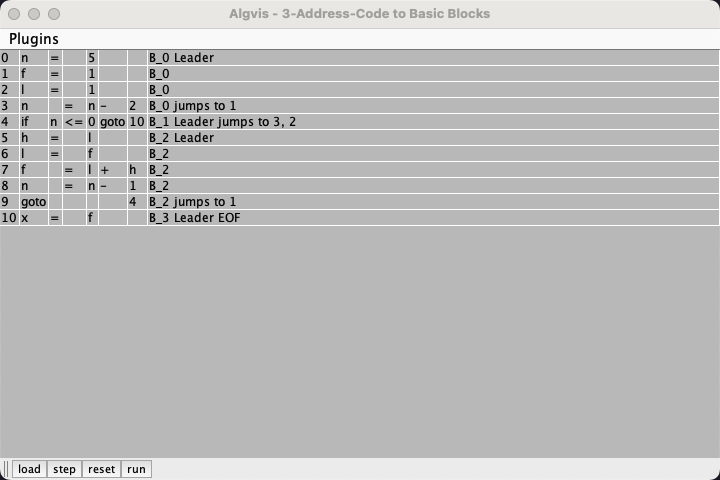
\includegraphics[width=0.8\textwidth]{fig/Screenshot_TacToBb.png}
  \caption{Das "3-Address-Code zu Grundblöcken" Plugin}
  \label{sc:TACtoBB}
\end{figure}
Dieses Plugin implementiert den in \cref{t:bb} eingeführten Algorithmus
und zeigt das 3-Address-Code Programm in einer Tabelle an (\cref{sc:TACtoBB}). Nach der
Ausführung des Programms wird in der Kommentarspalte der Tabelle für jede
Instruktion angezeigt zu welchem Grundblock sie gehört. Zudem wird auch angezeigt,
welche die folgenden Grundblöcke für jeden einzelnen Grundblock sind.

Dafür wird beim Erstellen eines Objektes der Algorithmusklasse 3-Address-Code
als String übergeben, ein \textit{ThreeAddressCode}-Objekt und ein Set erstellt, 
in welchem die gefundenen Leader gespeichert werden.

Durch das Aufrufen der \textit{step()}-Methode wird nun zwei Mal durch die
Instruktionen des \textit{ThreeAddressCode}-Objekts iteriert.

\newpage
Im ersten Durchlauf werden alle Leader markiert (\cref{cde:markLeaders}):
\begin{lstlisting}[language=Java, caption={Markieren von Leadern}, label={cde:markLeaders}]
ThreeAddressCodeInstruction instruction = code.get(address);
if(instruction.canJump()) {
  ThreeAddressCodeInstruction destination = code.get(
    Integer.parseInt(instruction.getDestination())
  );
  leaders.add(destination);
  destination.setComment("Leader");
  if(address+1 < code.size() 
  && instruction.getOperation() != ThreeAddressCodeOperation.jmp) {
    ThreeAddressCodeInstruction nextInstruction = code.get(address + 1);
    leaders.add(nextInstruction);
    nextInstruction.setComment("Leader");
  }
}
\end{lstlisting}

Im zweiten Durchlauf werden alle Instruktionen ihrem Block zugeordnet:
\begin{lstlisting}[language=Java, caption={Zuordnen der Instruktionen zu ihren Blöcken}, label={cde:mapBlocks}]
ThreeAddressCodeInstruction instruction = code.get(address);
if(leaders.contains(instruction)){
  int blockNumber = getSortedLeaders().indexOf(instruction);
  instruction.setComment("B_" + blockNumber + " Leader");
}else{
  ThreeAddressCodeInstruction lastLeader = getPreviousLeader(address);
  int blockNumber = getSortedLeaders().indexOf(instruction);
  instruction.setComment("B_" + blockNumber);
}

if(code.getLast().equals(instruction)) {
    ... // Kommentar wird mit Ziel des Sprungs ergaenzt
}else if(...) {
  ... // Dies wird im naechsten Plugin vollstaendig abgebildet
}

if(code.getLast().equals(instruction)) {
  instruction.setComment(instruction.getComment() + " EOF");
}
\end{lstlisting}
Hierbei ist die Methode \textit{getSortedLeaders()} eine Hilfsmethode, welche
das Set der erfassten Leader nach Adressen aufsteigend sortiert und als Liste wiedergibt.

\newpage
Im Kommentar-String jeder einzelnen Instruktion ist nun angegeben, in welchem
Block sich diese befindet, welche Instruktion Leader dieses Blockes ist und
zu welchen Blöcken die letzte Instruktion springt.\\
Um dies im Gui anzuzeigen, wird nach jeder Ausführung der \textit{step()}-Methode
die Methode \textit{refreshGuiElements()}(\cref{cde:refresh1}) in der Pluginklasse ausgeführt.
Diese aktualisiert alle Daten in der Tabelle und markiert dann die in diesem
Schritt betrachtete Zeile.
\begin{lstlisting}[language=Java, caption={Aktualisieren der Tabelle}, label={cde:refresh1}]
for (int i = 0; i < pluginInstance.getCode().size(); i++) {
  code.setRowTo(
    pluginInstance.getCode()
      .get(i)
      .getRepresentationAsStringArray()
    , i);
}
code.highlightLine(pluginInstance.getCurrentInstructionAddress());
\end{lstlisting}





\newpage
\subsection{Erstellung eines Kontrollflussgraphen aus 3-Address-Code}
\begin{figure}[h]
  \centering
  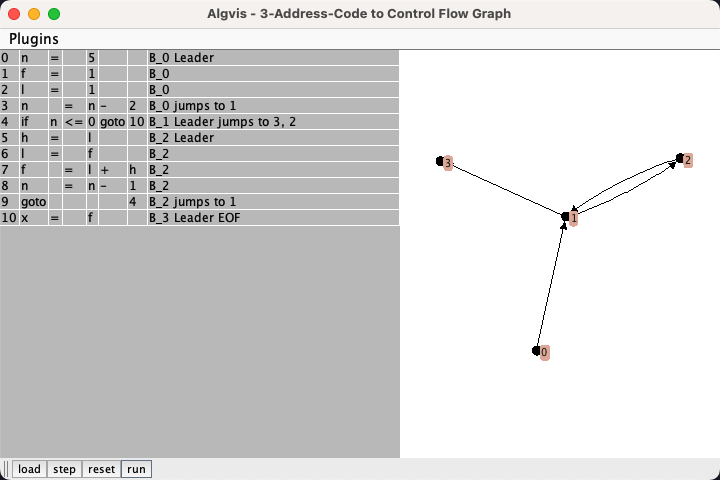
\includegraphics[width=0.8\textwidth]{fig/Screenshot_TacToCFG.png}
  \caption{Das "3-Address-Code zu Grundblöcken" Plugin}
  \label{fig:TACtoCFG}
\end{figure}

Das Plugin zur Generierung eines Kontrollflussgraphen aus 3-Address-Code 
ist eine Erweiterung des Plugins zur Erstellung von Grundblöcken.

Es erweitert das im letzten Abschnitt behandelte Programm indem es
neben der Tabelle einen Kontrollflussgraphen anzeigt.

Um dies zu realisieren, wurden neben einem Graphen, zwei Map-Objekte hinzugefügt. 
Eines in der Plugin-Klasse, um zu verfolgen, welche Grundblöcke bereits einen 
Knoten im Graphen besitzen und eines in der Algorithmus-Klasse, um festzuhalten,
welche Grundblöcke auf andere folgen.

Die Methode zum Zuordnen der Instruktionen zu ihren Grundblöcken (\cref{cde:mapBlocks})
wurde erweitert, sodass die Nachfolger der Grundblöcke nicht nur im Kommentar,
sondern auch in der Map erfasst werden:
\newpage
\begin{lstlisting}[language=Java, caption={Erweiterung der \textit{mapAddressesToItsBlock}-Methode}, label={cde:mapBlocks2}]
...
if(code.getLast().equals(instruction)) {
  if(instruction.canJump()){
    StringBuilder postfix = new StringBuilder(" jumps to ");
    ThreeAddressCodeInstruction nextInstruction = 
      instruction.nextPossibleInstructionAdresses().stream()
      .map(code::get)
      .min(ThreeAddressCodeInstruction::compareTo)
      .get();
    postfix.append(getSortedLeaders().indexOf(nextInstruction));
    successorMap.put(getPreviousLeader(address), new HashSet<>(Set.of(nextInstruction)));
    instruction.setComment(instruction.getComment() + postfix.toString());
  }
}else if(leaders.contains(code.get(address+1))) {
  StringBuilder postfix = new StringBuilder(" jumps to ");
  List<ThreeAddressCodeInstruction> nextInstructions = 
    instruction.nextPossibleInstructionAdresses().stream()
    .map(code::get)
    .toList();
  for (int i = 0; i < nextInstructions.size(); i++) {
    postfix.append(getSortedLeaders().indexOf(nextInstructions.get(i)));
    if(i+1<nextInstructions.size())
      postfix.append(", ");
  }
  successorMap.put(getPreviousLeader(address), new HashSet<>(nextInstructions));
  instruction.setComment(instruction.getComment() + postfix);
}

if(code.getLast().equals(instruction)) {
  instruction.setComment(instruction.getComment() + " EOF");
}
\end{lstlisting}
In den If Statements werden die Blöcke, in denen die Instruktionen die als nächstes
ausgeführt werden, ermittelt und an das Ende des Kommentars gehangen. Ausserdem
werden die Adressen der nächsten Instruktionen in die \textit{successorMap}
zugefügt
\footnote{Im Plugin \glqq 3-Address-Code to Basic Block\grqq\ existiert diese Map nicht, 
daher hat die Methode dort die beiden Befehle auch nicht.}.



\newpage
Die \textit{refreshGuiElements()}-Methode wurde auch um folgende Zeilen erweitert:
\begin{lstlisting}[language=Java, caption={Aktualisieren der Tabelle}, label={cde:refresh2}]
//set CFG
List<ThreeAddressCodeInstruction> leaders = 
  currentPluginInstance.getSortedLeaders();
for (ThreeAddressCodeInstruction leader : 
  currentPluginInstance.getSortedLeaders()) {
  //add new Nodes
  if(!nodeMap.containsKey(leader)) {
    Node node = new Node();
    nodeMap.put(leader, node);
    controlFlowGraph.addNode(nodeMap.get(leader));
  }
  controlFlowGraph.setLabelOfNode(
    nodeMap.get(leader), Integer.toString(leaders.indexOf(leader))
  );
}
//add all edges
Map<ThreeAddressCodeInstruction
  , Set<ThreeAddressCodeInstruction>> successorList = 
    currentPluginInstance.getSuccessorMap();
for (ThreeAddressCodeInstruction source:successorList.keySet()) {
  Node sourceNode = nodeMap.get(source);
  for (ThreeAddressCodeInstruction destination:
    successorList.get(source)) {
    Node destinationNode = nodeMap.get(destination);
    controlFlowGraph.addEdge(new Edge(sourceNode, destinationNode));
  }
}
\end{lstlisting}
In der ersten Schleife wird für jeden (bis zu diesem Schritt) 
gefundenen Leader ein Knoten im Graphen erstellt, wenn dieser 
noch nicht hinzugefügt worden ist. Das Label jedes Leaders aktualisiert,
da nicht zu jedem Zeitpunkt jeder Leader gefunden kann nicht davon ausgegangen werden,
dass die Label aus dem letzten Schritt noch aktuell sind.\\
In der zweiten Schleife werden für alle Leader Kanten zu den erkannten Nachfolgern gezeichnet.



\newpage
\subsection{Analyse von erreichenden Definitionen}
Das Plugin zur Visualisierung der Analyse der erreichenden Definitionen (\cref{fig:reachingDefinitions})
hat eine weitere Tabelle, in der Datenflusswerte angezeigt werden.
\begin{figure}[h]
  \centering
  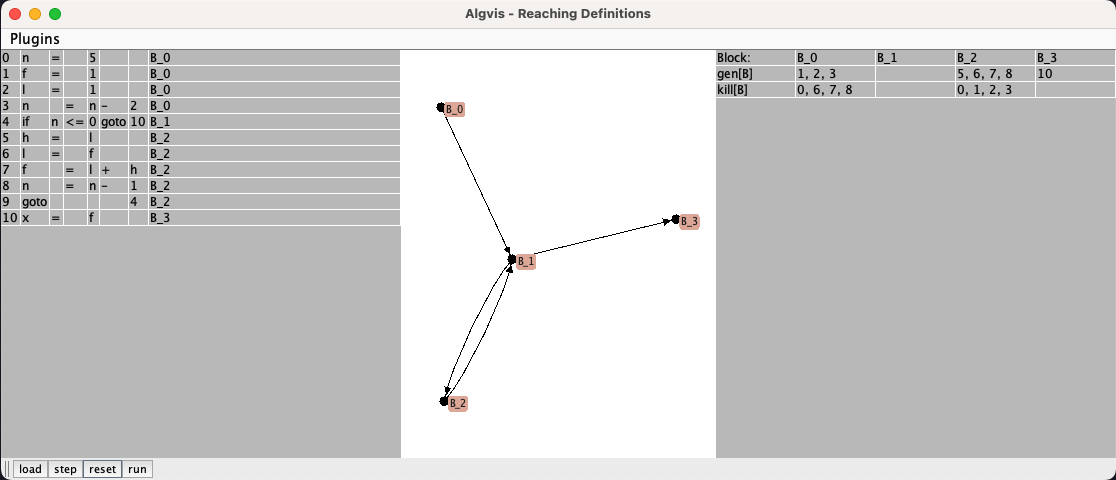
\includegraphics[width=0.99\textwidth]{fig/Screenshot_ReachingDefinitions.png}
  \caption{Das "Reaching Definitions" Plugin}
  \label{fig:reachingDefinitions}
\end{figure}

Da sich sowohl der Kontrollflussgraph, als auch der 3-Address-Code im
Verlaufe des Programmes nicht verändern, werden diese nicht in der
\textit{refreshGuiElements()}-Methode behandelt, sondern in der \textit{reset()}-Methode.
Da in dieser ein neues Objekt der Algorithmusklasse erstellt wird und
sich der Code nur dort ändern kann.

In der \textit{refreshGuiElements()}-Methode verändert sich dementsprechend
nur die Tabelle, in der Datenflusswerte angezeigt werden.

Diese berechnen wir, wie in \cref{t:rd} erläuftert, in der Algorithmusklasse:

Die $gen_B$ und $kill_B$-Mengen berechnen wir als Maps für jeden Grundblock $B$: 
\begin{lstlisting}[language=Java, caption={Berechnung einer $gen$ und $kill$-Menge}, label={cde:gen}]
//gen
Set<Integer> currentGenSet = gen.get(block);
for (int i = block.lastAddress(); i >= block.firstAddress(); i--) {
  ThreeAddressCodeInstruction currentInstruction = code.get(i);
  if(!currentInstruction.writesValue())
    continue;
  boolean newVar = true;
  for (int j : currentGenSet) {
    if(currentInstruction.getDestination().equals(code.get(j).getDestination()))
      newVar = false;
  }
  if(newVar)
    currentGenSet.add(i);
}
//kill
Set<Integer> currentKillSet = kill.get(block);
for (Integer i:currentGenSet) {
  for (int j = 0; j < code.size(); j++) {
    if(!code.get(j).writesValue())
      continue;
    if(j == i)
      continue;
    if(code.get(j).getDestination().equals(code.get(i).getDestination()))
      currentKillSet.add(j);
  }
}
\end{lstlisting}

Beim Durchlaufen des Algorithmus berechnen wir
in einem Schritt die $in[B]$ und $out[B]$ Mengen für einen Grundblock $B$.
Wenn diese sich von der in der letzten Iteration berechneten Menge
unterscheidet, ist unser Fixpunkt noch nicht erreicht.\\

Da wir nicht nur die aktuellen $in$ und $out$-Mengen darstellen wollen,
sondern alle, werden diese in einer Liste gespeichert.

Die $in_i[B]$-Menge wird als Vereinigung aller $out[B]$-Mengen der Vorgänger
des Blocks $B$ berechnet (\cref{cde:rdIn}):
\begin{lstlisting}[language=Java, caption={Berechnen der $in$-Menge}, label={cde:rdIn}]
Set<String> currentIn =  new HashSet<>();
for (BasicBlock ancestorBlock:ancestorBlocks) {
  Set<String> lastOut = (currentIteration>0) 
    ? out.get(currentIteration-1).get(ancestorBlock)
    : Set.of();//Leeres Set wenn es kein vorherige Iteration gibt
  currentIn.addAll(lastOut);
}
\end{lstlisting}

Die $gen_B$ und $kill_B$ Mengen wurden auf den Adressen der Instruktionen definiert,
werden jedoch als Adressen benötigt, daher werden sie wie folgt konvertiert:

\begin{lstlisting}[language=Java, caption={Konvertierung der $gen$-Menge}, label={cde:genConv}]
List<String> generatedIdentifiers = 
  gen.get(currentBlock).stream()
    .map(j -> code.get(j).getDestination())
    .toList();
List<String> killedIdentifiers = 
  kill.get(currentBlock).stream()
    .map(j -> code.get(j)
    .getDestination())
    .toList();
\end{lstlisting}

Um nun die $out[B]$-Menge zu berechen, werden alle Elemente der $kill_B$-Menge aus
einer Kopie der $in[B]$-Menge entfernt. Anschließend fügen wie alle Elemente der
$gen_B$-Menge hinzu:
\begin{lstlisting}[language=Java, caption={Berechnung der $out$-Menge}, label={cde:rdOut}]
Set<String> currentOut = new HashSet<>(currentIn);
currentOut.removeAll(killedIdentifiers);
currentOut.addAll(generatedIdentifiers);
\end{lstlisting}

Um die berechneten Datenflusswerte anzuzeigen, wird die Tabelle 
wie im Beispiel (\cref{tab:fib-rd}) befüllt:

Die erste Zeile dient als Überschriftszeile für die Grundblöcke.
Die zweite und dritte Zeile befüllen die $gen_B$ und $kill_B$ Mengen(\cref{cde:visgenkill}):
\begin{lstlisting}[language=Java, caption={Berechnung der $out$-Menge}, label={cde:visgenkill}]
dataFlow.setValueAt("gen[B]", 1, 0);
dataFlow.setValueAt("kill[B]", 2, 0);
for (int col = 0; col < basicBlocks.size(); col++) {
  BasicBlock block = basicBlocks.get(col);
  String genBlock = collectStringSet(
    pluginInstance.getGen().get(block).stream()
      .map(String::valueOf)
      .collect(Collectors.toSet())
    );
  String killBlock = collectStringSet(
    pluginInstance.getKill().get(block).stream()
      .map(String::valueOf)
      .collect(Collectors.toSet())
    );
  dataFlow.setValueAt(genBlock, 1, col+1);
  dataFlow.setValueAt(killBlock, 2, col+1);
}
\end{lstlisting}
Die Methode \textit{collectStringSet} ist hier eine Helfermethode, welche ein
Set an Strings zu einem String kombiniert, indem die einzelnen Elemente durch Kommas getrennt werden.

In den folgenden Zeilen werden die $in[B]$ und $out[B]$ Mengen aufgelistet.
Da in der letzten Iteration eventuell noch nicht alle Mengen bestimmt worden sind, 
wird für die unbestimmten Mengen ein Platzhalter-Set mit dem Element \glqq -\grqq  eingefügt:

\begin{lstlisting}[language=Java, caption={Visualisierung der $in$ und $out$-Mengen}, label={cde:visinout}]
for (int i = 0; i < inTable.size();i++) {
  int rowIndex = (i*2)+3;
  Map<BasicBlock, Set<String>> inMap = inTable.get(i);
  Map<BasicBlock, Set<String>> outMap = outTable.get(i);
  dataFlow.setValueAt("in[B]^"+i, rowIndex, 0);
  dataFlow.setValueAt("out[B]^"+i, rowIndex+1, 0);
  for (int j = 0; j < basicBlocks.size(); j++) {
    Set<String> inBlock = inMap.getOrDefault(basicBlocks.get(j), Set.of("-"));
    String inString = collectStringSet(inBlock);
    dataFlow.setValueAt(inString, rowIndex, j+1);

    Set<String> outBlock = outMap.getOrDefault(basicBlocks.get(j), Set.of("-"));
    String outString = collectStringSet(outBlock);
    dataFlow.setValueAt(outString, rowIndex+1, j+1);
  }
}
\end{lstlisting}

\newpage
\subsection{Analyse von lebendigen Variablen bezüglich Grundblöcken}
\begin{figure}[h]
  \centering
  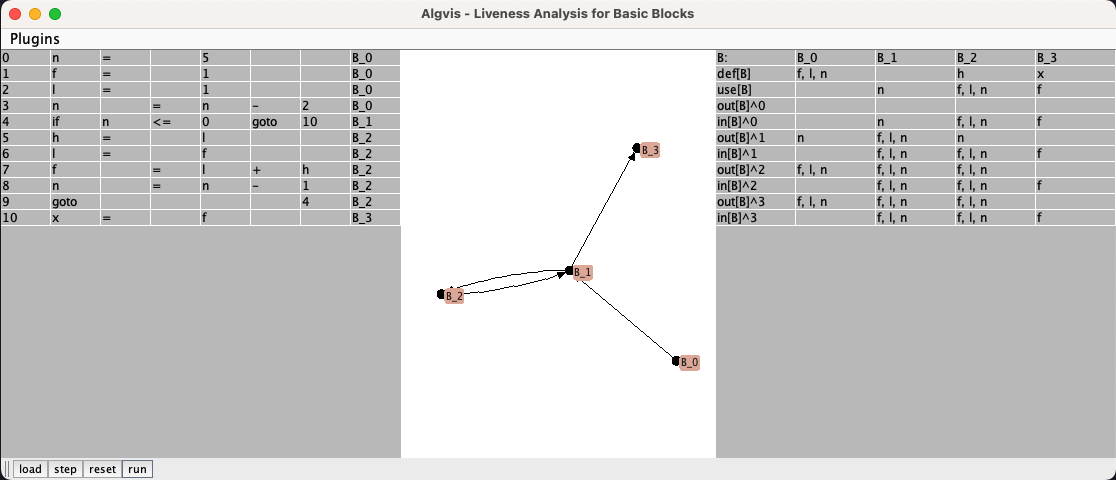
\includegraphics[width=0.99\textwidth]{fig/Screenshot_LivenessBb.png}
  \caption{Das "Liveness Analysis for Basic Blocks" Plugin}
  \label{fig:livenessAnalysisBB}
\end{figure}
Im folgenden Kapitel wird die Implementation des Algorithmus für die Liveness
Analysis besprochen. Da der Aufbau der Gui identisch zu dem Plugin für errichende
Definitionen ist, wird darauf nicht erneut eingegangen.

Da die Datenflussrichtung rückwärts läuft, wird die $out[B]$-Menge wie folgt
bestimmt:
\begin{lstlisting}[language=Java, caption={Berechnung der $out$-Menge}, label={cde:laIn}]
Set<String> currentOut = new HashSet<>();
for (BasicBlock successor:successorBlocks) {
  Set<String> lastInSuccessor = (currentIteration>0)
    ? in.get(currentIteration-1).get(successor)
    : Set.of();
  currentOut.addAll(lastInSuccessor);
}
\end{lstlisting}

\newpage
Um den Algorithmus wie in \cref{t:la} zu implementieren, müssen für alle
Grundblöcke $B$ die $def_B$ und $use_B$ Mengen definiert werden.
Dies geschieht wie folgt (\cref{cde:laDefUse}):
\begin{lstlisting}[language=Java, caption={Berechnung der $def$ und $use$-Mengen}, label={cde:laDefUse}]
//def
Set<String> currentDefSet = def.get(block);
for (int i = block.lastAddress(); i >= block.firstAddress(); i--) {
  ThreeAddressCodeInstruction instruction = code.get(i);
  if(!instruction.writesValue())
    continue;
  String identifier = instruction.getDestination();
  currentDefSet.add(identifier);
  for (int j = 0; j < i; j++) {
    if(code.get(j).getUsedIdentifiers().contains(identifier))
      currentDefSet.remove(identifier);
  }
}
//use
Set<String> currentUseSet = use.get(block);
for (int i = block.lastAddress(); i >= block.firstAddress(); i--) {
  ThreeAddressCodeInstruction instruction = code.get(i);
  for (String used:instruction.getUsedIdentifiers()) {
    currentUseSet.add(used);
    for (int j = block.firstAddress(); j < i; j++) {
      if(code.get(j).writesValue() && code.get(j).getDestination().equals(used))
        currentUseSet.remove(used);
    }
  }
}
\end{lstlisting}
Und die Transferfunktion wird wie folgt berechnet:

\begin{lstlisting}[language=Java, caption={Berechnung der $out$-Menge}, label={cde:laOut}]
Set<String> currentIn = new HashSet<>(currentOut);
currentIn.removeAll(def.get(currentBlock));
currentIn.addAll(use.get(currentBlock));
\end{lstlisting}

\newpage
\subsection{Analyse von lebendigen Variablen bezüglich einzelnen Instruktionen}
\begin{figure}[h]
  \centering
  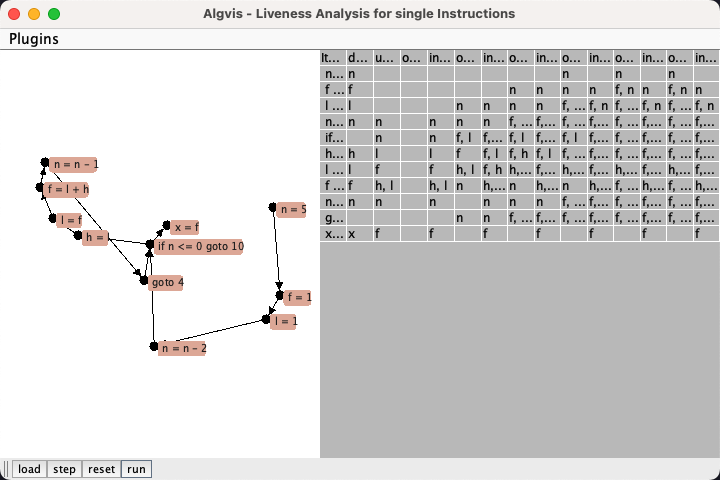
\includegraphics[width=0.8\textwidth]{fig/Screenshot_LivenesTAC.png}
  \caption{Das "Liveness Analysis for Three Address Code" Plugin}
  \label{fig:livenessAnalysisTAC}
\end{figure}
Durch die im letzten Abschnitt definierte Liveness Analyse lässt sich mit wenigen
Iterationen eine konservative Abschätzung der benötigten Register machen.
Da sich jedoch auch innerhalb eines Grundblocks die Werte der Liveness Analyse ändern können,
kann die liveness Analyse auch auf einzelnen Instruktionen geführt werden, 
hierbei werden jedoch wesentlich mehr Iterationen benötigt, bis der Fixpunkt erreicht ist.\\

Dieses Plugin (\cref{fig:livenessAnalysisTAC}) implementiert eben diese Analyse. Indem es alle Instruktionen
in einem Graphen anzeigt und deren Datenflusswerte in einer Tabelle.

Die Transferfunktion bleibt identisch zur liveness Analyse auf Grundblöcken.
Jedoch müssen die $use_i$ und $def_i$-Mengen auf einzelnen Instruktionen $i$
definiert werden:
\begin{itemize}
  \item Die $use_i$-Menge umfasst trivialer Weise alle Adressen die in ihrer Instruktion $i$
    benötigt werden.
  \item Die $def_i$-Menge ist definiert durch: 
    Alle Instruktionen, die einen Wert definieren haben ein Element in ihrer
    $def_i$ Menge, nämlich die Adresse in der dieser Wert gespeichert wird.
    Wenn eine Instruktion keinen Wert speichert, gilt $def_i=\emptyset$.
\end{itemize}
